\section{Experiments}
\label{sec:experiments}


%%%%%%%%%%%%%%%%%%%%%%%%%%%%%%%%%%%%%%%%%%%%%%%%%%%%%%%%%%%%
%%%%%%%%%% PU Learning
%%%%%%%%%%%%%%%%%%%%%%%%%%%%%%%%%%%%%%%%%%%%%%%%%%%%%%%%%%%%

\subsection{Learning with only positive and unlabeled samples}
\label{subsec:pulearning}


In this section, we apply the sigmoid/softmax loss for the negative class to train classifiers with only positive data and unlabeled data and compare with the class-weighted loss regarding the learned decision boundary, the achieved precision and recall.

\subsubsection{2D non-linear dataset}

To investigate the decision boundaries led by the sigmoid loss for the negative class, we trained a multilayer perceptron with a two-dimensional, non-linear separable dataset.

\paragraph{Dataset}
The training data contains four hundred samples per class drawn randomly from two interleaving half circles with noises added with a minor standard deviation, as shown in Figure \ref{fig:moons}.
Half of the positive examples were assigned negative labels, resulting in a training data with reliable positive labels but noisy negative labels.


\paragraph{Experimental setup}
The multilayer perceptron contains two layers, with six neurons per layer.
The normal logistic loss, the class-weighted logistic loss, and the class-dependent sigmoid loss were trained independently, and the result optimal decision boundaries are drawn as white regions in Figure \ref{fig:moons}.
The same multilayer perceptron classifier was also trained with true labels to present a baseline decision boundary.
The weights for the positive class and the negative class in the weighted logistic loss were 1 and 0.5 respectively.

\paragraph{Decision boundary with large margin by the sigmoid loss}
If trained with the sigmoid loss, the decision boundary is distant from the positive cluster with a relatively large margin, whereas the decision boundary for the weighted logistic loss is still closed to the positive examples, as shown in Figure \ref{fig:moons}.
For sigmoid loss, the mislabeled positive examples far away from the decision boundary do not contribute more loss than samples less distant from the decision boundary.
As a consequence, the loss derivative with respect to the model weights is larger for examples near the decision boundary than examples far away, illustrated as marker sizes in Figure \ref{fig:moonsdiff}.
The derivative determines the update rate for the model weights.
Higher derivative means a higher rate of update.
Therefore, examples near the decision boundary have a higher contribution to the model updates for the sigmoid loss.
In other words, the sigmoid loss emphasizes the positive predictions with low confidence.
The emphasization of the uncertain predictions near the decision boundary for the sigmoid loss leads to a decision boundary converges to low-density regions for the inputs distribution.
By contrast, the logistic loss has higher derivative for positive predictions with high confidence.
It emphasizes the incorrect predictions with confidence so that the decision boundary is pulled toward the positive cluster by mislabeled positive samples.
Since the sigmoid loss converges to an optimal decision boundary that has a relatively large margin from the positive cluster while still keeping distant from the negative samples, it is expected to achieve high recall and not sacrifice precision.


%%%%%%%% FIGURE MOONS

\begin{figure*}
\begin{center}
\textbf{Classifier decision boundaries with different losses}\par\medskip
% \fbox{\rule{0pt}{2in} \rule{.9\linewidth}{0pt}}
   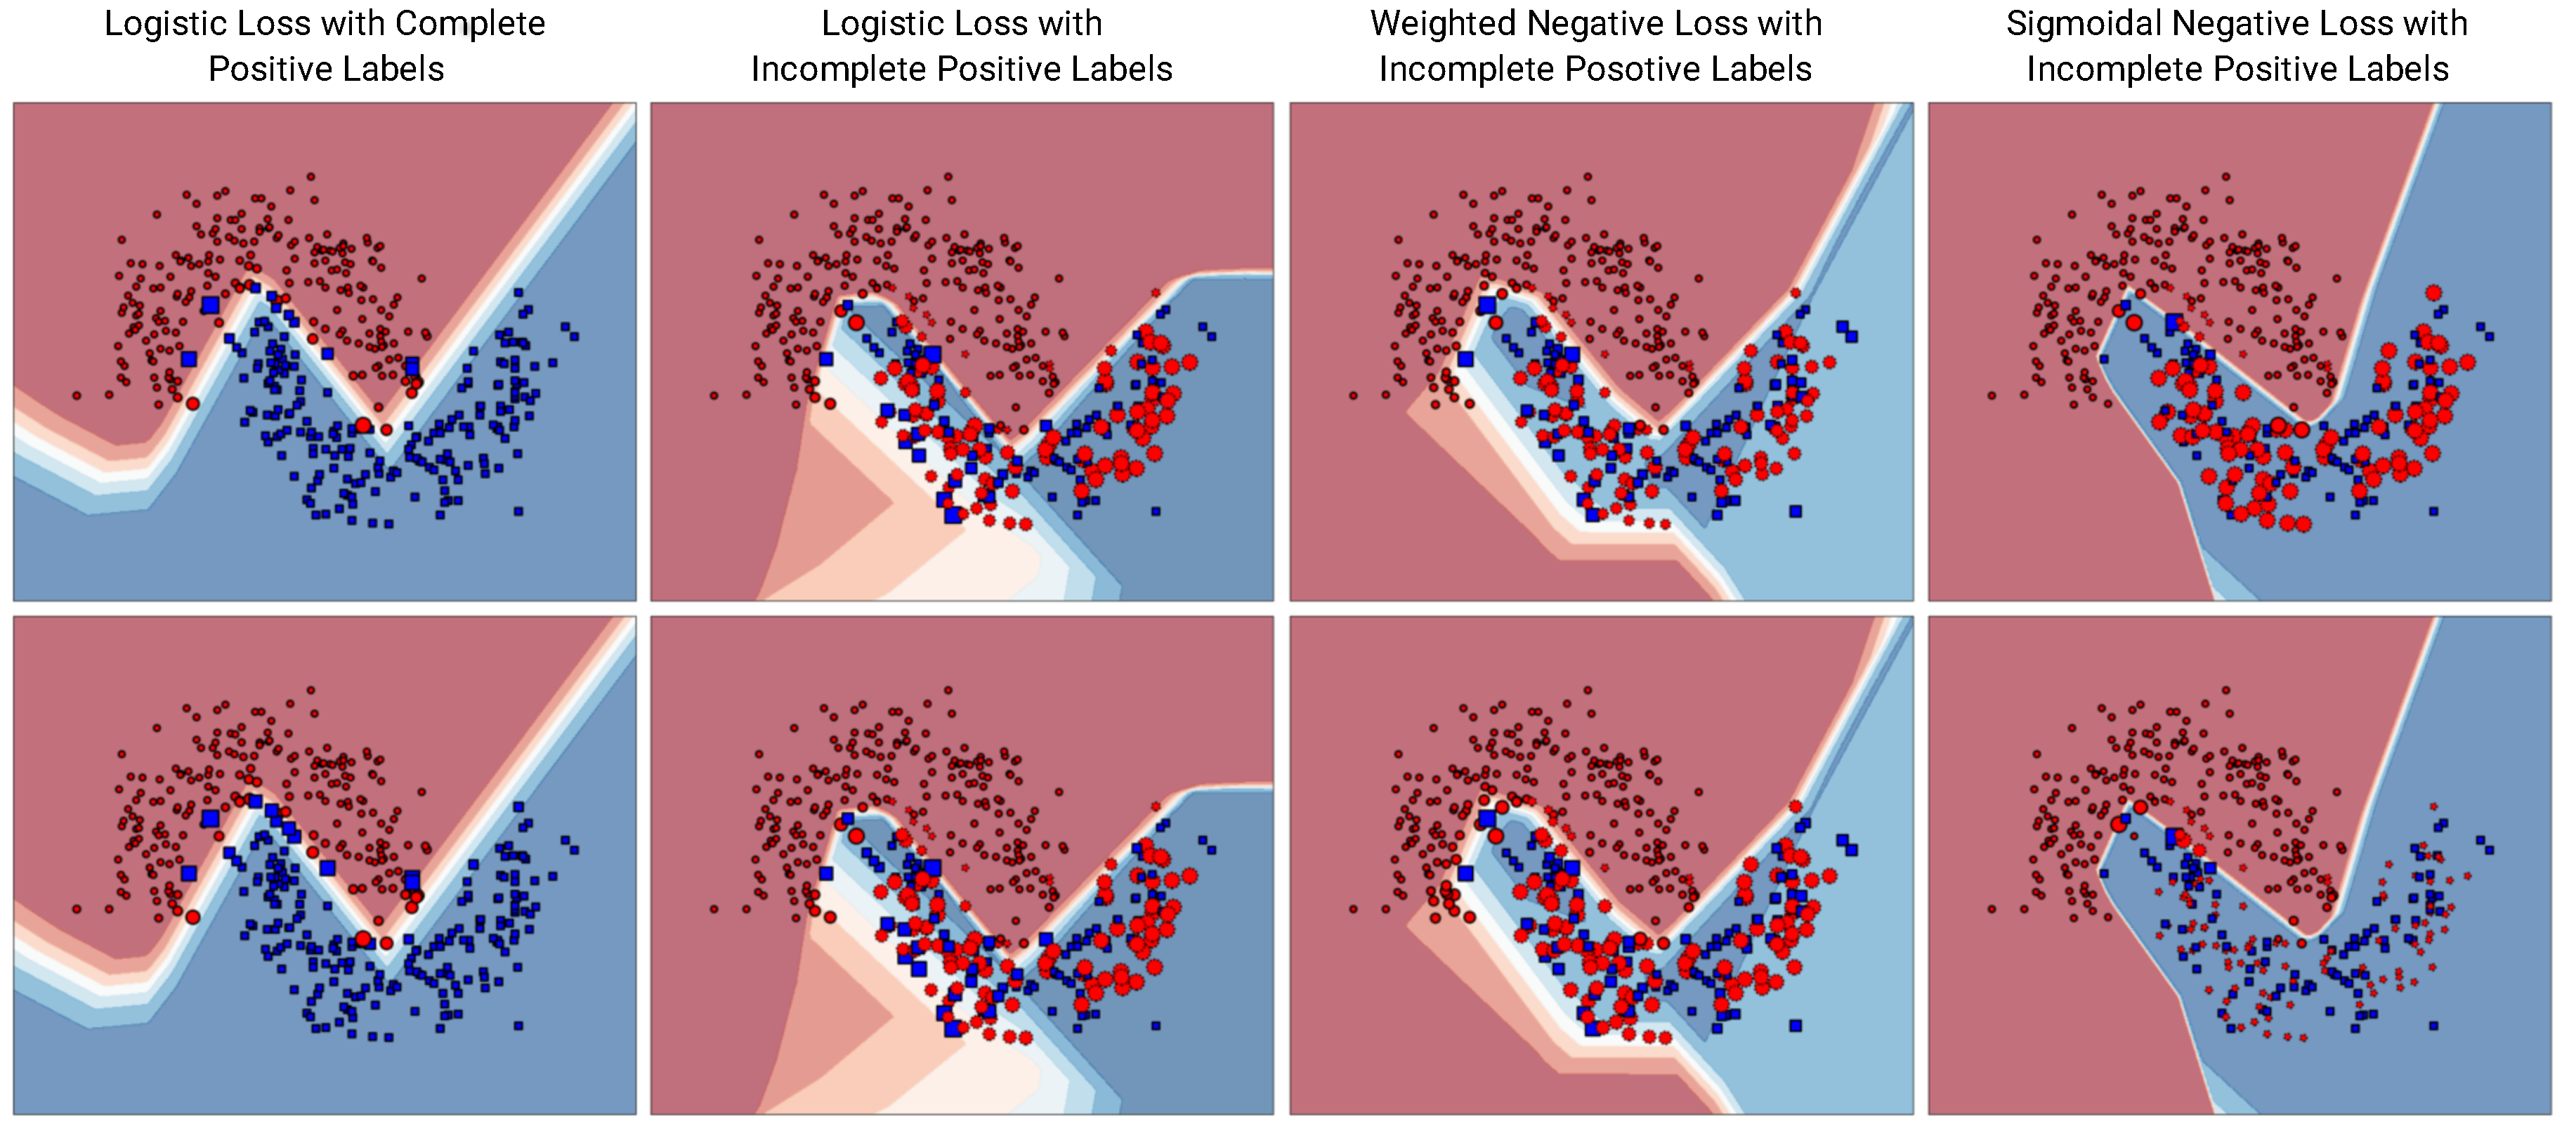
\includegraphics[width=0.95\linewidth]{img/moons.pdf}
\end{center}
   \caption{
   Decision boundaries of a 2-layer multilayer perceptron trained with different losses on a 2D moons dataset with the unlabeled positive.
  %%  The \textbf{leftmost} figures have complete positive labels, meaning the positive and negative labels are all correct, whereas, in \textbf{the other figures} only half of the positives were correctly labeled and the rest were mixed with the negative samples.
   A \textbf{red circle} represents an example labeled as positive and a \textbf{blue square} represents the example has a negative label.
   The \textbf{background colors} indicate the classifier prediction in the corresponding area: \textbf{red} for negative class, \textbf{blue} for positive class and \textbf{white} for the class transition areas, i.e., decision boundaries.
   The \textbf{markers sizes} demonstrates the training loss normalized per-class.
   Compared to the normal logistic loss and weighted logistic loss (positive:negative=1:0.5), the decision boundary optimized with the sigmoid loss has a large margin from the positive cluster as well as from the negative clusters.
   It is expected to achieve both high recall and high precision.
   (Best viewed in color.)
   }
\label{fig:moons}
\end{figure*}


\begin{figure}[t]
\begin{center}
\textbf{Derivatives of different losses and decision boundaries}\par\medskip
   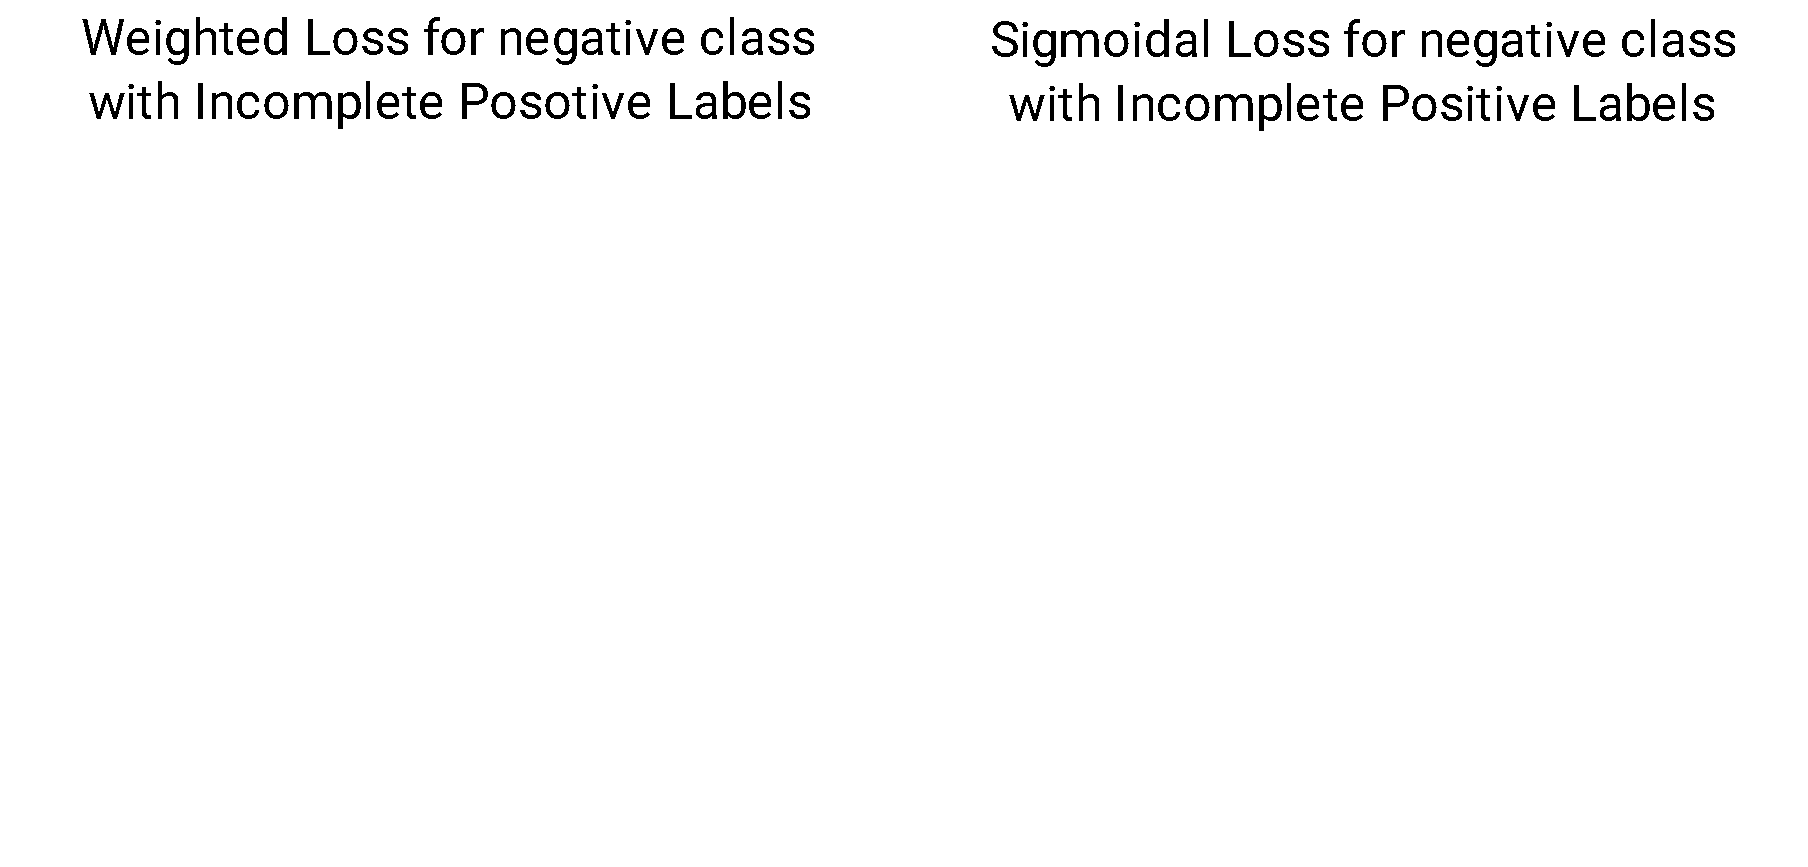
\includegraphics[width=\linewidth]{img/moons_diff}
\end{center}
   \caption{
   Derivatives w.r.t the last layer output for the two losses (normalized per class and shown as the marker size).
   The sigmoid loss has small derivatives for samples farther from the decision boundary and large derivatives for samples near the decision boundary, which is opposite to the weighted logistic loss.
   Higher derivative means the example has a higher rate to update the model weights during optimization.
   The sigmoid loss emphasizes the uncertain incorrect predictions (points near the decision boundary) in training, whereas the weighted logistic loss emphasizes the confident incorrect predictions (points distant from the decision boundary).
   (Best viewed in color.)
   }
\label{fig:moonsdiff}
\end{figure}



\subsubsection{CIFAR dataset}

To compare the precision and recall achieved by the class-dependent sigmoid/softmax loss and the class-weighted loss, we trained a CNN model to classify images of multiple relevant categories from non-relevant images with partially labeled relevant images.

\paragraph{Dataset}
We combined the CIFAR10 dataset and CIFAR100 dataset \cite{krizhevsky2009learning} to form a dataset with images for eleven classes: ten relevant classes from CIFAR10 and one non-relevant class for all categories from CIFAR100.
Only part of the relevant images are labeled (with correct classes), and the rest of the relevant images forms an unlabeled (U) set together with the non-relevant images.
Images from the unlabeled set were assigned negative labels.

\paragraph{Experimental setup}
An eight layer CNN model was trained with the cross-entropy loss, the class-weighted cross-entropy loss and the class-depend sigmoid loss respectively in the simulated PU learning setup, where 50\% of the positive examples were unlabeled.
The CNN model was also trained with the modified hard bootstrapping loss introduced in Section \ref{sec:pulearning} to set a benchmark for the state-of-the-art method to learn in the presence of label noises.
Model performances were evaluated on a separate test set with true labels.
The architecture of the CNN model can be found in Table \ref{tab:8layer} in Appendix \ref{subsec:8layer}.
Each model was trained from scratch with Adam optimizer and base learning rate 0.0001.
Experiments were repeated three times with random split of P set, and U set and standard deviations were around 0.01 if not explicitly mentioned.
% Note that there is no category overlap between CIFAR10 dataset and CIFAR100 dataset.

%%%%%%%% TABLE CIFAR10 50%

\paragraph{Higher recall and comparable precision with the softmax loss}

Table \ref{tab:cifar} shows using the softmax loss for the non-relevant class achieves better recall than the class-weighted cross-entropy loss without lowering precision significantly.
With 50\% of the relevant examples correctly labeled and the rest assigned non-relevant labels, the normal cross-entropy loss leads to an imbalanced model with high precision but low recall, and therefore with a low f1-score.
By reweighing the loss for the non-relevant class by a factor of 0.5, the model becomes balanced for precision and recall so that the result f1-score is improved significantly.
Compared to the class-weighted cross entropy, the class-dependent softmax loss improves recall by 0.08 while reduces precision only by 0.01.
The f1-score achieved by the class-dependent softmax loss is slightly better than the class-weighted loss, though not as good as training with clean labels with either 50\% of the sample or the complete training set.
The state-of-the-art benchmark method, the hard bootstrap loss, achieves the same f1-score as the softmax loss but not as high recall.
The softmax loss for the non-relevant class can achieve higher recall without sacrificing the precision by much, compared to the class-weighted loss.

% It is noteworthy that the weighted negative loss and hard bootstrapping loss achieved more balanced precision and recall than the sigmoid negative loss.
% That is because the two former losses were weighted by classes frequency of observed labels, around 0.67 for the negative class and 2 for positive classes, whereas the sigmoid negative loss was not.
% Reweighing the sigmoid negative loss by observed label frequencies would trade too much precision for recall (0.74 and 0.83 respectively), resulting in a worse f1-score than not reweighing losses.
% The sigmoid negative loss seems to be easier over-balancing with the same choice of class weights.
% Besides, the optimal precision and recall for sigmoid negative loss seem more unstable which may relate to the nonconvex class-dependent loss.


\begin{table}[t]
\centering
\textbf{Classification performance with partially labeled relevant data}\par\medskip
\resizebox{\columnwidth}{!}{
\centering
\begin{tabular}{ll|llll}
Annotation  & Loss & acc. & mean prec. & mean rec. & mean $F_1$ \\
\hline
R+N         & CrossEntropy   & 0.87 & 0.88 & 0.82 & 0.85 \\
50\%(R+N)   & CrossEntropy   & 0.83 & 0.84 & 0.78 & 0.80 \\
50\%R+U     & CrossEntropy   & 0.66 & 0.94 & 0.38 & 0.49 \\
\hline
50\%R+U     & ClassWeighted     & 0.78 & 0.75 & 0.75 & 0.76 \\
50\%R+U     & SoftmaxLoss      & 0.79 & 0.74 & \textbf{0.83} & \textbf{0.78} \\
50\%R+U     & BootstrapHard    & \textbf{0.80} & 0.76 & 0.81 & \textbf{0.78} \\
\end{tabular}
}
\caption{
Comparing different losses for training a 2-layer multilayer perception to classify ten relevant classes and one non-relevant class with partially labeled relevant examples and unlabeled non-relevant examples.
The trained classifiers are evaluated on a test set of true labels.
For each of the relevant classes, precision, recall, and f1-score are measured with the one-vs-all strategy and averaged.
\textbf{R+N} denotes model trained with the complete relevant labels (R set) and non-relevant labels (N set);
\textbf{50\%(R+N)} represents model trained with the half of the relevant labels and non-relevant labels respectively;
\textbf{50\%R+U} means the model is trained with half of the relevant samples, and the rest relevant samples are mixed with non-relevant samples (U set).
Weighting the non-relevant class for the cross-entropy loss by a factor of 0.5 improves the mean f1-score significantly.
The class-dependent softmax loss achieves higher recall than the class-weighted loss without sacrificing precision, but not as good as training with a set of labeled negative examples (R+N and 50\%(R+N)).
% The class-dependent softmax loss performs similar to the hard bootstrapping loss, with a higher recall but slightly lower accuracy.
The class-dependent softmax loss achieves better f1-score than the class-weighted loss and is comparable to a state-of-the-art method, the hard bootstrapping loss.
}
\label{tab:cifar}
\end{table}


%%%%%%%% FIGURE Varying positive annotating percetage
To compare the class-dependent softmax loss and the class-weighted cross entropy with varying percentage of labeled relevant images, we also trained models with datasets containing varing percentages of labeled relevant images.
Figure \ref{fig:pct_annotating} demonstrates that the class-dependent softmax loss performs slightly better than the class-weighted cross-entropy when the percentage of labeled relevant images is neither too high ($>0.8$) nor too low ($<0.2$).
When the percentage of labeled relevant images is high or low, the softmax loss behaves no worse than the class-weighted cross-entropy.
Therefore, the sigmoid loss is in general better than weighting the losses for different classes.
% When the labeled percentage of relevant images is high, the difference in loss contributions of the unlabeled relevant images for the two losses is small.
% When the percentage is low, the severe imbalance of classes introduced by unlabeled relevant images prevents the models from achieving good classification performance.

% Similarly as the result at 50\% positive examples labeled, the sigmoid loss and the hard bootstrapping loss have only little improvement compared to the weighted negative loss.
% The assumption we made for the sigmoid negative loss was that the probability of a negative example being wrong is dependent on the confidence.
% However, the synthesized mislabeled positive examples were distributed at random when we synthesized them, meaning that the probability for a negative label being wrong is independent of the underlying distribution of the inputs.
% No matter where the decision boundary is, such uniformly distributed incorrect negative labels are independent of the prediction confidence.
% Therefore, it is expected for the sigmoid negative loss and bootstrapping loss to have similar performance as the weighted negative loss.

% By varying the percentage of labeled relevant examples, the class-dependent sigmoid loss performs slightly better than the class weighted cross-entropy when the percentage of the labeled relevant images is neither too high (>0.8) nor too low (<0.2), as shown in Figure \ref{fig:pct_annotating}.
% Besides, FIgure \ref{fig:pct_annotating} demonstrates that learning with a subset of explicitly labeled non-relevant examples (RN setup) outperforms learning with the mixed unlabeled examples (RU setup) for any percentage of labeled positives and any losses being used.
% This result is expected because the explicitly labeled non-relevant examples deliver extra information about which images in the unlabeled set are non-relevant.
% Therefore, learning with positive and unlabeled examples is only relevant when it is impossible to easily construct a subset of negative examples from the unlabeled data.
% Otherwise, training with true positive and negative labels, and potentially with semi-supervised learning, would be superior to training with positive and unlabeled examples only.

\begin{figure}[t]
\centering
\textbf{Classification performance with varying percentage of labeled relevant images}\par\medskip
\centering
   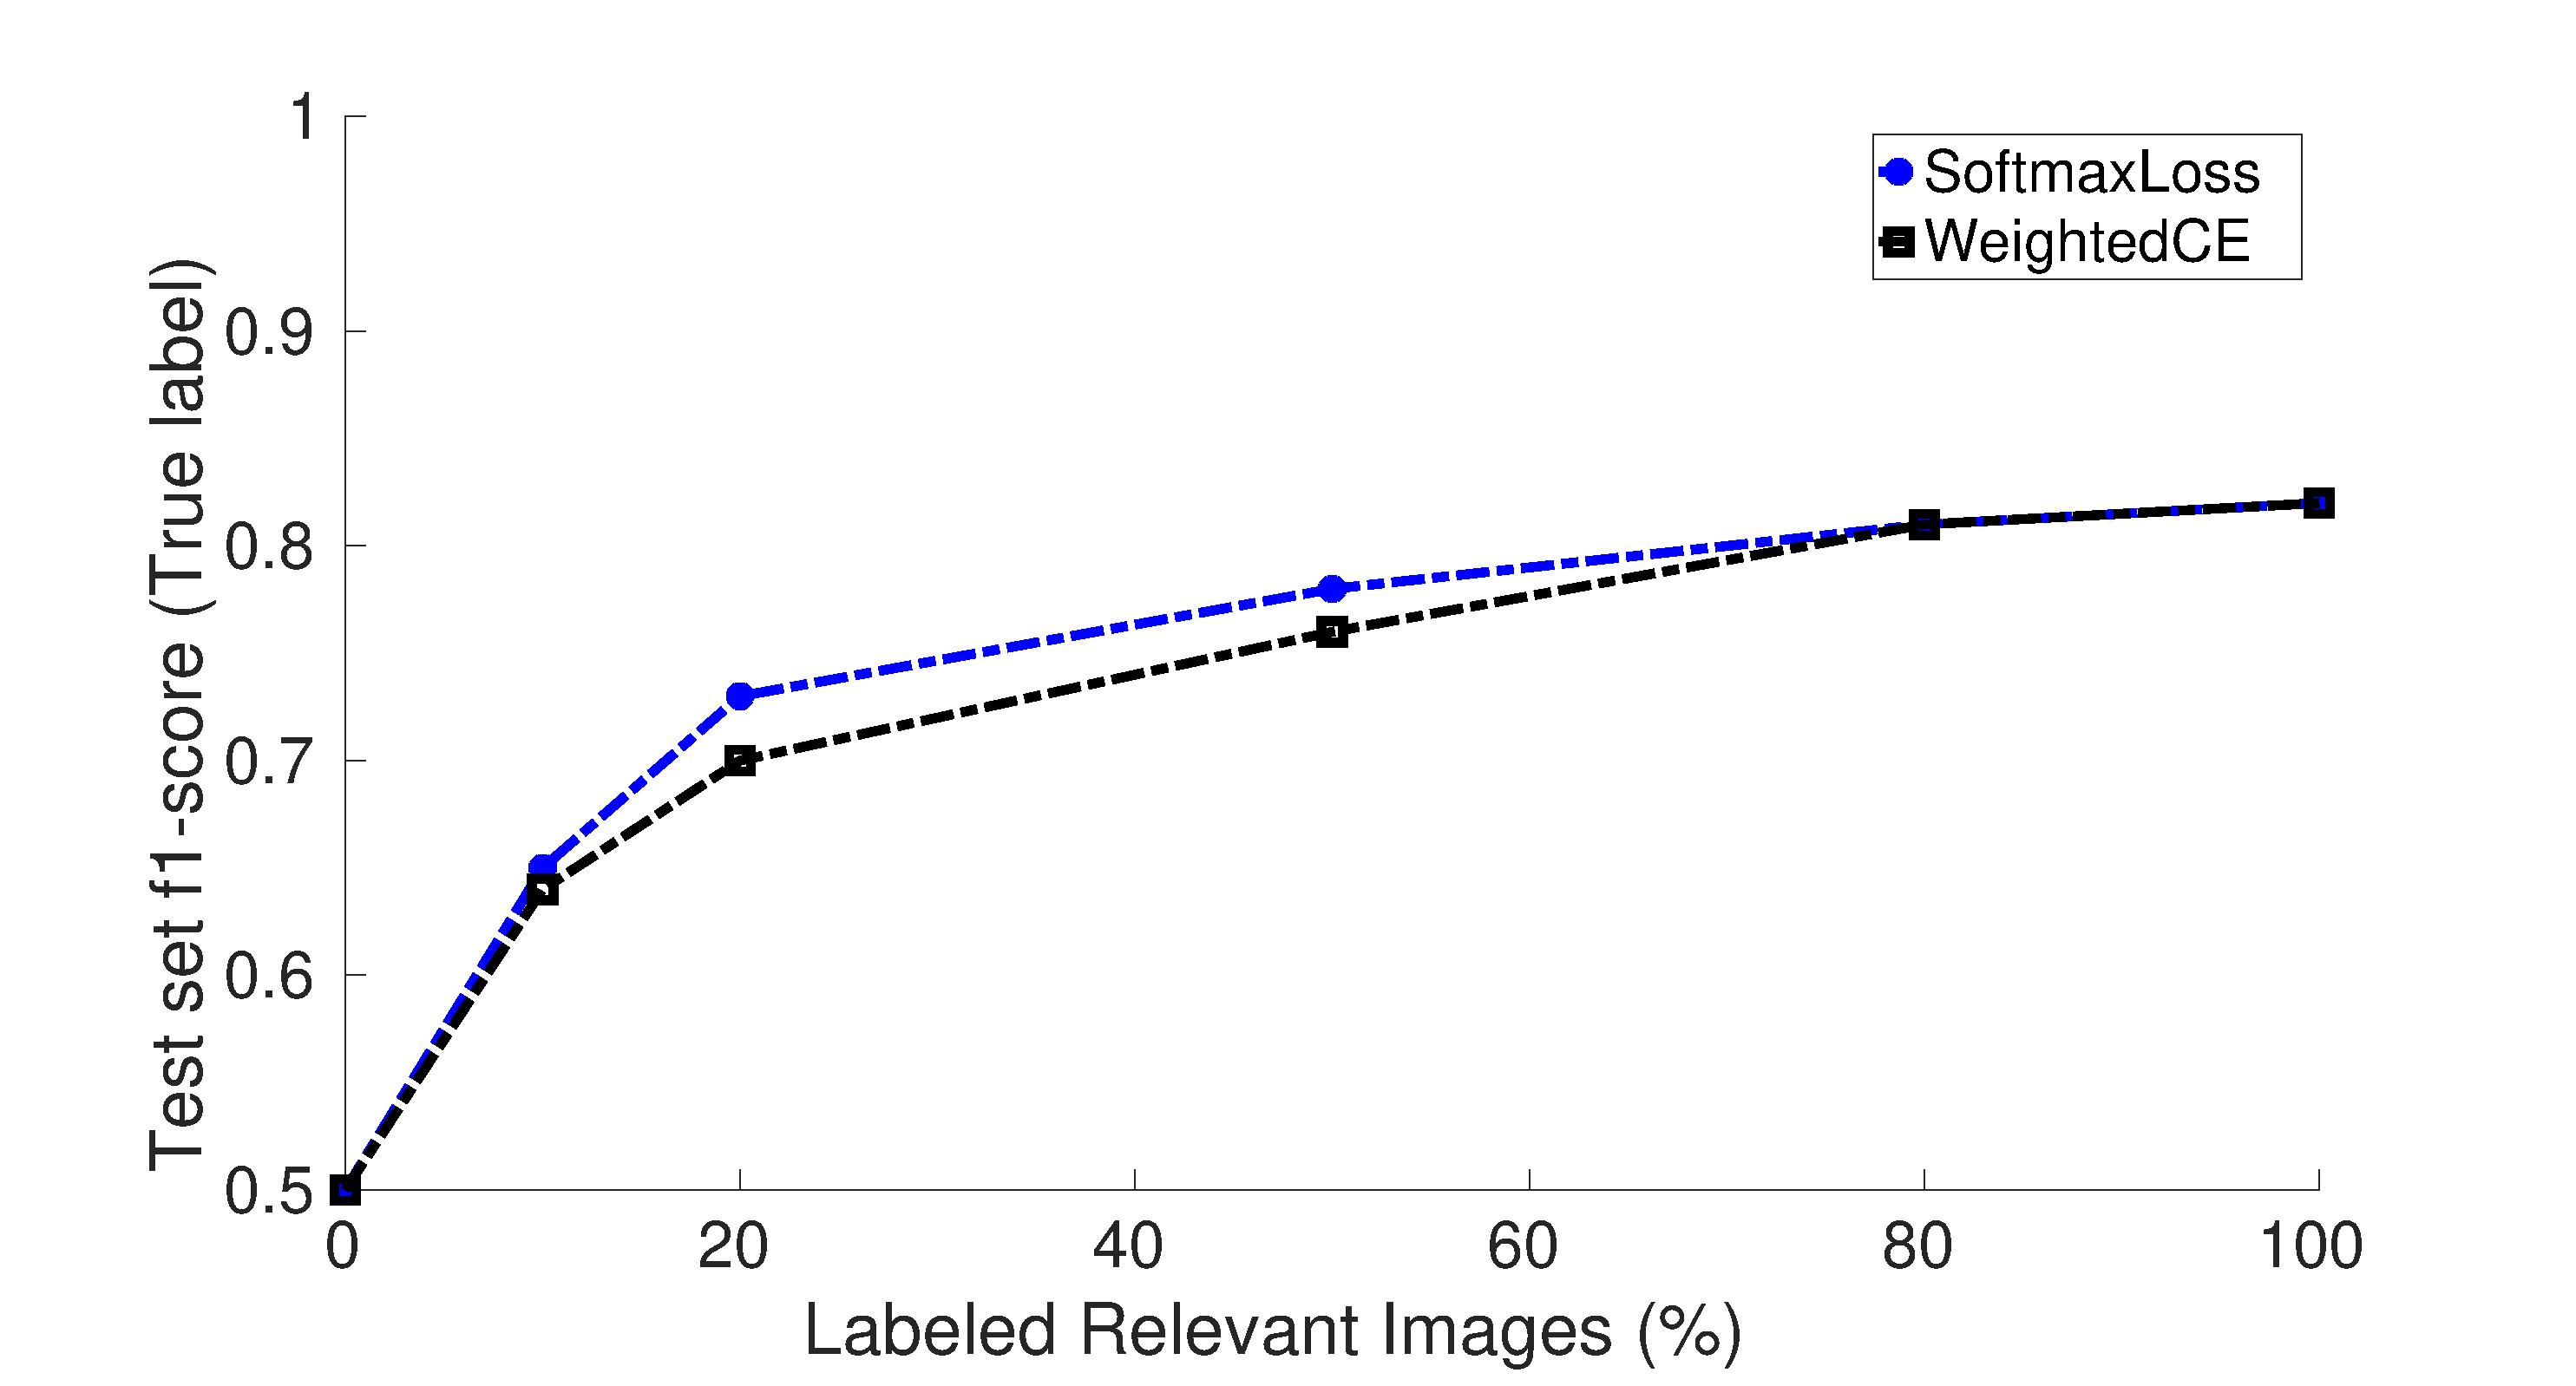
\includegraphics[width=1.05\linewidth]{img/pu_vs_pn}
\caption{
Comparing f1-score for the class-dependent softmax loss and the class-weighted cross entropy with varying percentage of relevant images labeled.
% \textbf{R+N} represents training with a percentage of reliable, relevant labels and non-relevant labels, while \textbf{R+U} stands for training with a percentage of relevant labels and all other images as unlabeled.
The class-dependent softmax loss achieves better test f1-score than the class-weighted cross entropy when 20\% and 50\% percentage of relevant images are labeled, and the others are mixed with non-relevant images.
% The class-dependent sigmoid loss achieves slightly higher f1-score than the weighted cross-entropy loss at labeled relevant  20\% and 50\% of the relevant samples are labeled.
% In general, training with explicitly labeled non-relevant examples (RN) is superior to training with an unlabeled set of mixed relevant and non-relevant examples (RU).
}
\label{fig:pct_annotating}
\end{figure}


%%%%%%%% Text Segmentation Pascal VOC2011
\subsection{Learning with incomplete segmentations}
\label{subsec:incomplete}
To compare the class-dependent sigmoid loss with the class-weighted logistic loss for training foreground/background segmentation with incomplete segmentations, we constructed an incompletely labeled dataset from the PASCAL VOC2011 dataset \cite{everingham2015pascal} with extra segmentations \cite{hariharan2011semantic}.

\paragraph{Dataset}
Objects from the 20 foreground categories of the PASCAL VOC2011 dataset were labeled as foreground, constructing binary segmentations with the background pixels.
We selected objects in the training images completed at random with a probability of 0.5 to be labeled.
The other objects and the background pixels were left unlabeled.
Only single-object images were used for training and testing to avoid the influence of two adjacent objects joining as one object because of binary segmentation, resulting in totally 4000 training images for 20 categories available for pre-training, fine-tuning and evaluation.
We subsampled the original images by four times to accelerate the training process.


\paragraph{Experimental setup}
A Fully Convolutional Networks with AlexNet model (FCN-AlexNet), as shown in Figure \ref{fig:fcn} in Appendix \ref{subsec:segmentation}, was used for experiments because of its relatively small capacity and thus short training time.
The FCN-AlexNet model was trained together with the normal logistic loss, the class-weighted logistic loss, and the class-dependent sigmoid loss independently to predict binary segmentation, determining whether a pixel is a foreground or background.
The learned models were evaluated with the test set of the PASCAL VOC2011 dataset with complete binary segmentations.
Weights from the pre-trained AlexNet model \cite{krizhevsky2012imagenet} were used as initialization for compatible weights of the FCN-AlexNet model.
The other weights of the FCN-AlexNet model were randomly initialized with Xavier initialization \cite{glorot2010understanding}.
The default hyperparameters of FCN-AlexNet in \cite{long2015fully} were kept unchanged.
The training process run 240,000 iterations for pre-training phase, and 12,000 iterations for fine-tuning phase.
Snapshots for trained models were taken every 4,000 iterations.
Each experiment was repeated three times, and the highest mean IU achieved on the test set for the last five snapshots were summarized in Table \ref{tab:pusegment}.


\paragraph{Higher recall with the sigmoid loss}
As shown in Table \ref{tab:pusegment}, the class dependent sigmoid loss achieves the higher mean recall by approximately 0.07 than training with the normal logistic loss, and by 0.04 than the class-weighted loss.
% The performance of training with sigmoid loss and 50\% objects unsegmented is still not comparable to training with complete segmentations.
Specifically for the two classes, the foregorund recall class increases whereas the background recall decreases for the sigmoid loss.
This difference in classes lead to a mean IU for the class-dependent sigmoid loss no better than the class-weigthed loss because the mean IU counts for both low false positive rate and low false negative rate.
% The sigmoid loss increases precision for recall, similarly as observed in training the CIFAR dataset.
The class-dependent sigmoid loss improves the recall averaged for the foreground class and background class when training with incomplete segmentations.

%%%%%%%% TABLE Segmentation Pascal VOC2011
\begin{table}[t]
\centering
\textbf{Segmentation performance}\par\medskip
\resizebox{\columnwidth}{!}{
\centering
\begin{tabular}{ll|llll}
Annotation  & Loss & overall acc. & mean rec. & f.w. IU & mean IU \\
\hline
% Complete            & CrossEnt.U       &  0.88 & 0.60 & 0.48 & 0.80 \\
% 50\%Unsegmented     & CrossEnt.U       &  0.83 & 0.31 & 0.27 & 0.70 \\
% 50\%Unsegmented     & WeightedU        &  0.83 & 0.34 & 0.29 & 0.70 \\
% 50\%Unsegmented     & ExponentialU     &  0.83 & 0.34 & 0.29 & 0.70 \\
Complete       & LogisticLoss       &  0.90 & 0.85 & 0.82 & 0.75 \\
50\%Unseg.     & LogisticLoss       &  0.85 & 0.68 & 0.73 & 0.60 \\
50\%Unseg.     & ClassWeighted       &  0.84 & 0.71 & 0.73 & \textbf{0.62} \\
50\%Unseg.     & SigmoidLoss      &  0.83 & \textbf{0.75} & 0.72 & \textbf{0.62} \\
\end{tabular}
}
\caption{
Training foreground/background segmentation with different losses when 50\% of the objects are unsegmented.
The performances are achieved on the test set of PASCAL VOC2011 segmentation dataset.
% A class weight of 0.7:1.75 was used to balance the sample frequency differences of the two classes.
% The negative loss was further weighted by a factor of 0.5 for the weighted negative loss.
% Mean accuracy is equivalent to the average recall over the two classes.
% Mean IU is the average intersection over union ratio (IU) over two classes and f.w. IU is the frequency weighted average of IU over the two classes.
Both the class-dependent sigmoid loss and the class-weighted logistic loss perform better than the normal logistic loss when 50\% objects unsegmented, but not as good as the model trained with complete segmentations.
The class-dependent sigmoid loss achieves higher recall than the class-weighted logistic loss and a similar mean IU as the class-weighted logistic loss.
}
\label{tab:pusegment}
\end{table}


%%%%%%%% Figure Segmentation Pascal VOC2011
Selective predictions made by the models trained with the sigmoid loss and the cross entropy loss were presented in Figure \ref{fig:pusegment}.
For the two example images shown, the model trained with the cross entropy loss failed to segment objects from images whereas the sigmoid loss predicted segmentations on the position of the objects.
The coarse outlines were mainly due to the limited compacity of the FCN-AlexNet model.
The third column shows predictions given by model trained with complete training segmentation, and it did not produce more accurate outlines than training with the sigmoid loss and incomplete segmentations.
There is no example observed correctly segmented by the model with the class-weighted logistic loss but not by the model with the class-dependent sigmoid loss.
These two examples show that the sigmoid loss improves the segmentation performance by segment a few more objects than the weighted logistic loss.

\begin{figure}[t]
\centering
\textbf{Example predictions}\par\medskip
  \begin{minipage}{\columnwidth}\footnotesize
  \centering
  \subsubfloat{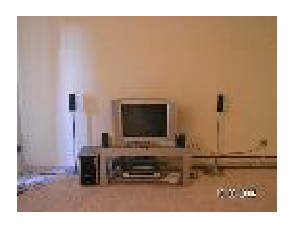
\includegraphics[width=0.19\columnwidth]{img/2007_002132}}{Raw}
  \subsubfloat{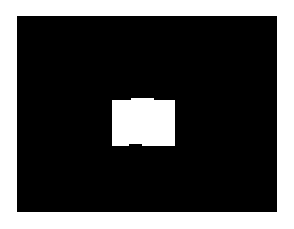
\includegraphics[width=0.19\columnwidth]{img/2007_002132_label}}{Label}
  \subsubfloat{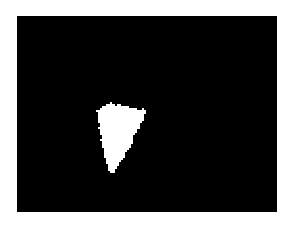
\includegraphics[width=0.19\columnwidth]{img/2007_002132_up_pred}}{Complete}
  \subsubfloat{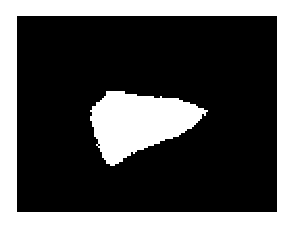
\includegraphics[width=0.19\columnwidth]{img/2007_002132_exp_pred}}{SigmoidLoss}
  \subsubfloat{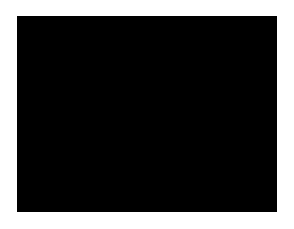
\includegraphics[width=0.19\columnwidth]{img/2007_002132_low_pred}}{ClassWeight.}
  \subsubfloat{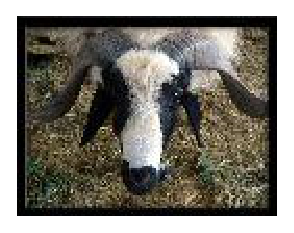
\includegraphics[width=0.19\columnwidth]{img/2007_002618}}{Raw}%
  \subsubfloat{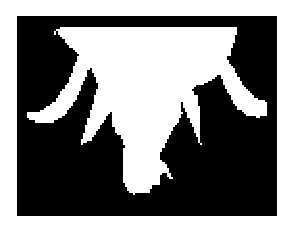
\includegraphics[width=0.19\columnwidth]{img/2007_002618_label}}{Label}
  \subsubfloat{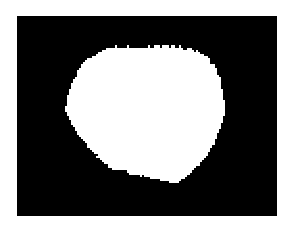
\includegraphics[width=0.19\columnwidth]{img/2007_002618_up_pred}}{Complete}
  \subsubfloat{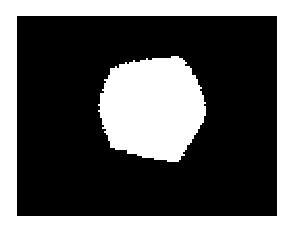
\includegraphics[width=0.19\columnwidth]{img/2007_002618_exp_pred}}{SigmoidLoss}
  \subsubfloat{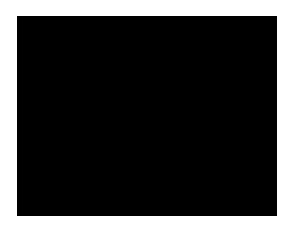
\includegraphics[width=0.19\columnwidth]{img/2007_002618_low_pred}}{ClassWeight.}
  \end{minipage}
\caption{
Example predictions made by models trained with the logistic loss and the class-dependent sigmoid loss.
This figure presents two selective images for which the model trained with the logistic loss failed to segment objects, whereas the model trained with the class-dependent sigmoid negative loss succeed.
}
\label{fig:pusegment}
\end{figure}

%%%%%%%%%%%%%%%%%%%%%%%%%%%%%%%%%%%%%%%%%%%%%%%%%%%%%%%%%%%%
%%%%%%%%%% Label noises
%%%%%%%%%%%%%%%%%%%%%%%%%%%%%%%%%%%%%%%%%%%%%%%%%%%%%%%%%%%%


%%%%%%%%%%%%%%%%%%%%%%%%%%%%%%%%%%%%%%%%%%%%%%%%%%%%%%%%%%%%
%%%%%%%% Table Objects mislabelling
%%%%%%%%%%%%%%%%%%%%%%%%%%%%%%%%%%%%%%%%%%%%%%%%%%%%%%%%%%%%
\begin{table*}[t]
\centering
\textbf{Fine-tuning performance of representations trained in the presence of random labels}\par\medskip
\resizebox{\textwidth}{!}{
\centering
\begin{tabular}{l|c|cccc|c}

\hline
\multirow{2}{*}{}                                                               & \multirow{2}{*}{\begin{tabular}[c]{@{}c@{}}Pre-trained\\ Models\end{tabular}} & \multicolumn{4}{c|}{Fine-tuning mean IU per pretraining-finetuning fold}                                                                       & \multirow{2}{*}{\begin{tabular}[c]{@{}l@{}}Average \\ mean IU\end{tabular}} \\ \cline{3-6}
                                                                                &                                                                               & Fold1                             & Fold2                             & Fold3                             & Fold4                              &                                                                             \\ \hline
\multirow{2}{*}{Baseline}                                                       & RandomWeights                                                                 & \multicolumn{1}{c}{$0.29\pm0.01$} & \multicolumn{1}{c}{$0.29\pm0.03$} & \multicolumn{1}{c}{$0.27\pm0.01$} & \multicolumn{1}{c|}{$0.30\pm0.02$} & \multicolumn{1}{c}{$0.29\pm0.02$}                                           \\
                                                                                & TrueLabels                                                                    & \multicolumn{1}{c}{$0.29\pm0.01$} & \multicolumn{1}{c}{$0.36\pm0.01$} & \multicolumn{1}{c}{$0.29\pm0.01$} & \multicolumn{1}{c|}{$0.37\pm0.01$} & \multicolumn{1}{c}{$\mathbf{0.33\pm0.01}$}                                  \\ \hline
\multirow{3}{*}{\begin{tabular}[c]{@{}l@{}}Objects \\ Mislabelling\end{tabular}}      & AllRandomLabels                                                     & $0.29\pm0.01$                                                                                           & $0.33\pm0.03$                                                                               & $0.26\pm0.01$                                                                                                  & $0.28\pm0.01$                                                                                           & $0.29\pm0.01$                                                                                                          \\
                                                                                      & HalfRandomLabels                                                    & $0.27\pm0.01$                                                                                           & $0.33\pm0.02$                                                                               & $0.25\pm0.01$                                                                                                  & $0.29\pm0.01$                                                                                           & $0.29\pm0.01$                                                                                                          \\
                                                                                      & BinarizedLabels                                                     & $0.30\pm0.02$                                                                                           & $0.35\pm0.01$                                                                               & $0.29\pm0.02$                                                                                                  & $0.35\pm0.03$                                                                                           & $\mathbf{0.32\pm0.02}$                                                                                                 \\ \hline

\end{tabular}
}
\caption{
Segmentation performance for FCN-AlexNet models pre-trained on 15 categories from the PASCAL VOC2011 dataset and fine-tuned on the other five categories.
The splits of pre-training and fine-tuning categories are organized in four folds.
\textbf{RandomWeights} represents the randomly initialized weights;
\textbf{TrueLabels} stands for the model pre-trained with true labels;
\textbf{AllRandomLabels} denotes the model pre-trained with all random foreground labels;
\textbf{HalfRandomLabels} is the model pre-trained with half random and half correct foreground labels;
\textbf{BinaryLabels} demonstrates that the model is pre-trained with binary (foreground and background) segmentations;
Random foreground labels for segmentations in the training set decreased the fine-tuning performance for the learned representations, compared to the true foreground labels.
Training foreground and background segmentation instead of per foreground class segmentation improves the fine-tuning performance when the pre-training dataset contains mislabeled objects from one foreground class to another.
}
\label{tab:random}
\end{table*}




%%%%%%%%%%%%%%%%%%%%%%%%%%%%%%%%%%%%%%%%%%%%%%%%%%%%%%%%%%%%
%%%%%%%% Figure categorizing classes
%%%%%%%%%%%%%%%%%%%%%%%%%%%%%%%%%%%%%%%%%%%%%%%%%%%%%%%%%%%%

\begin{figure}[t]
\centering
\textbf{Fine-tuning performance of representations trained with categorized segmentation labels}\par\medskip
   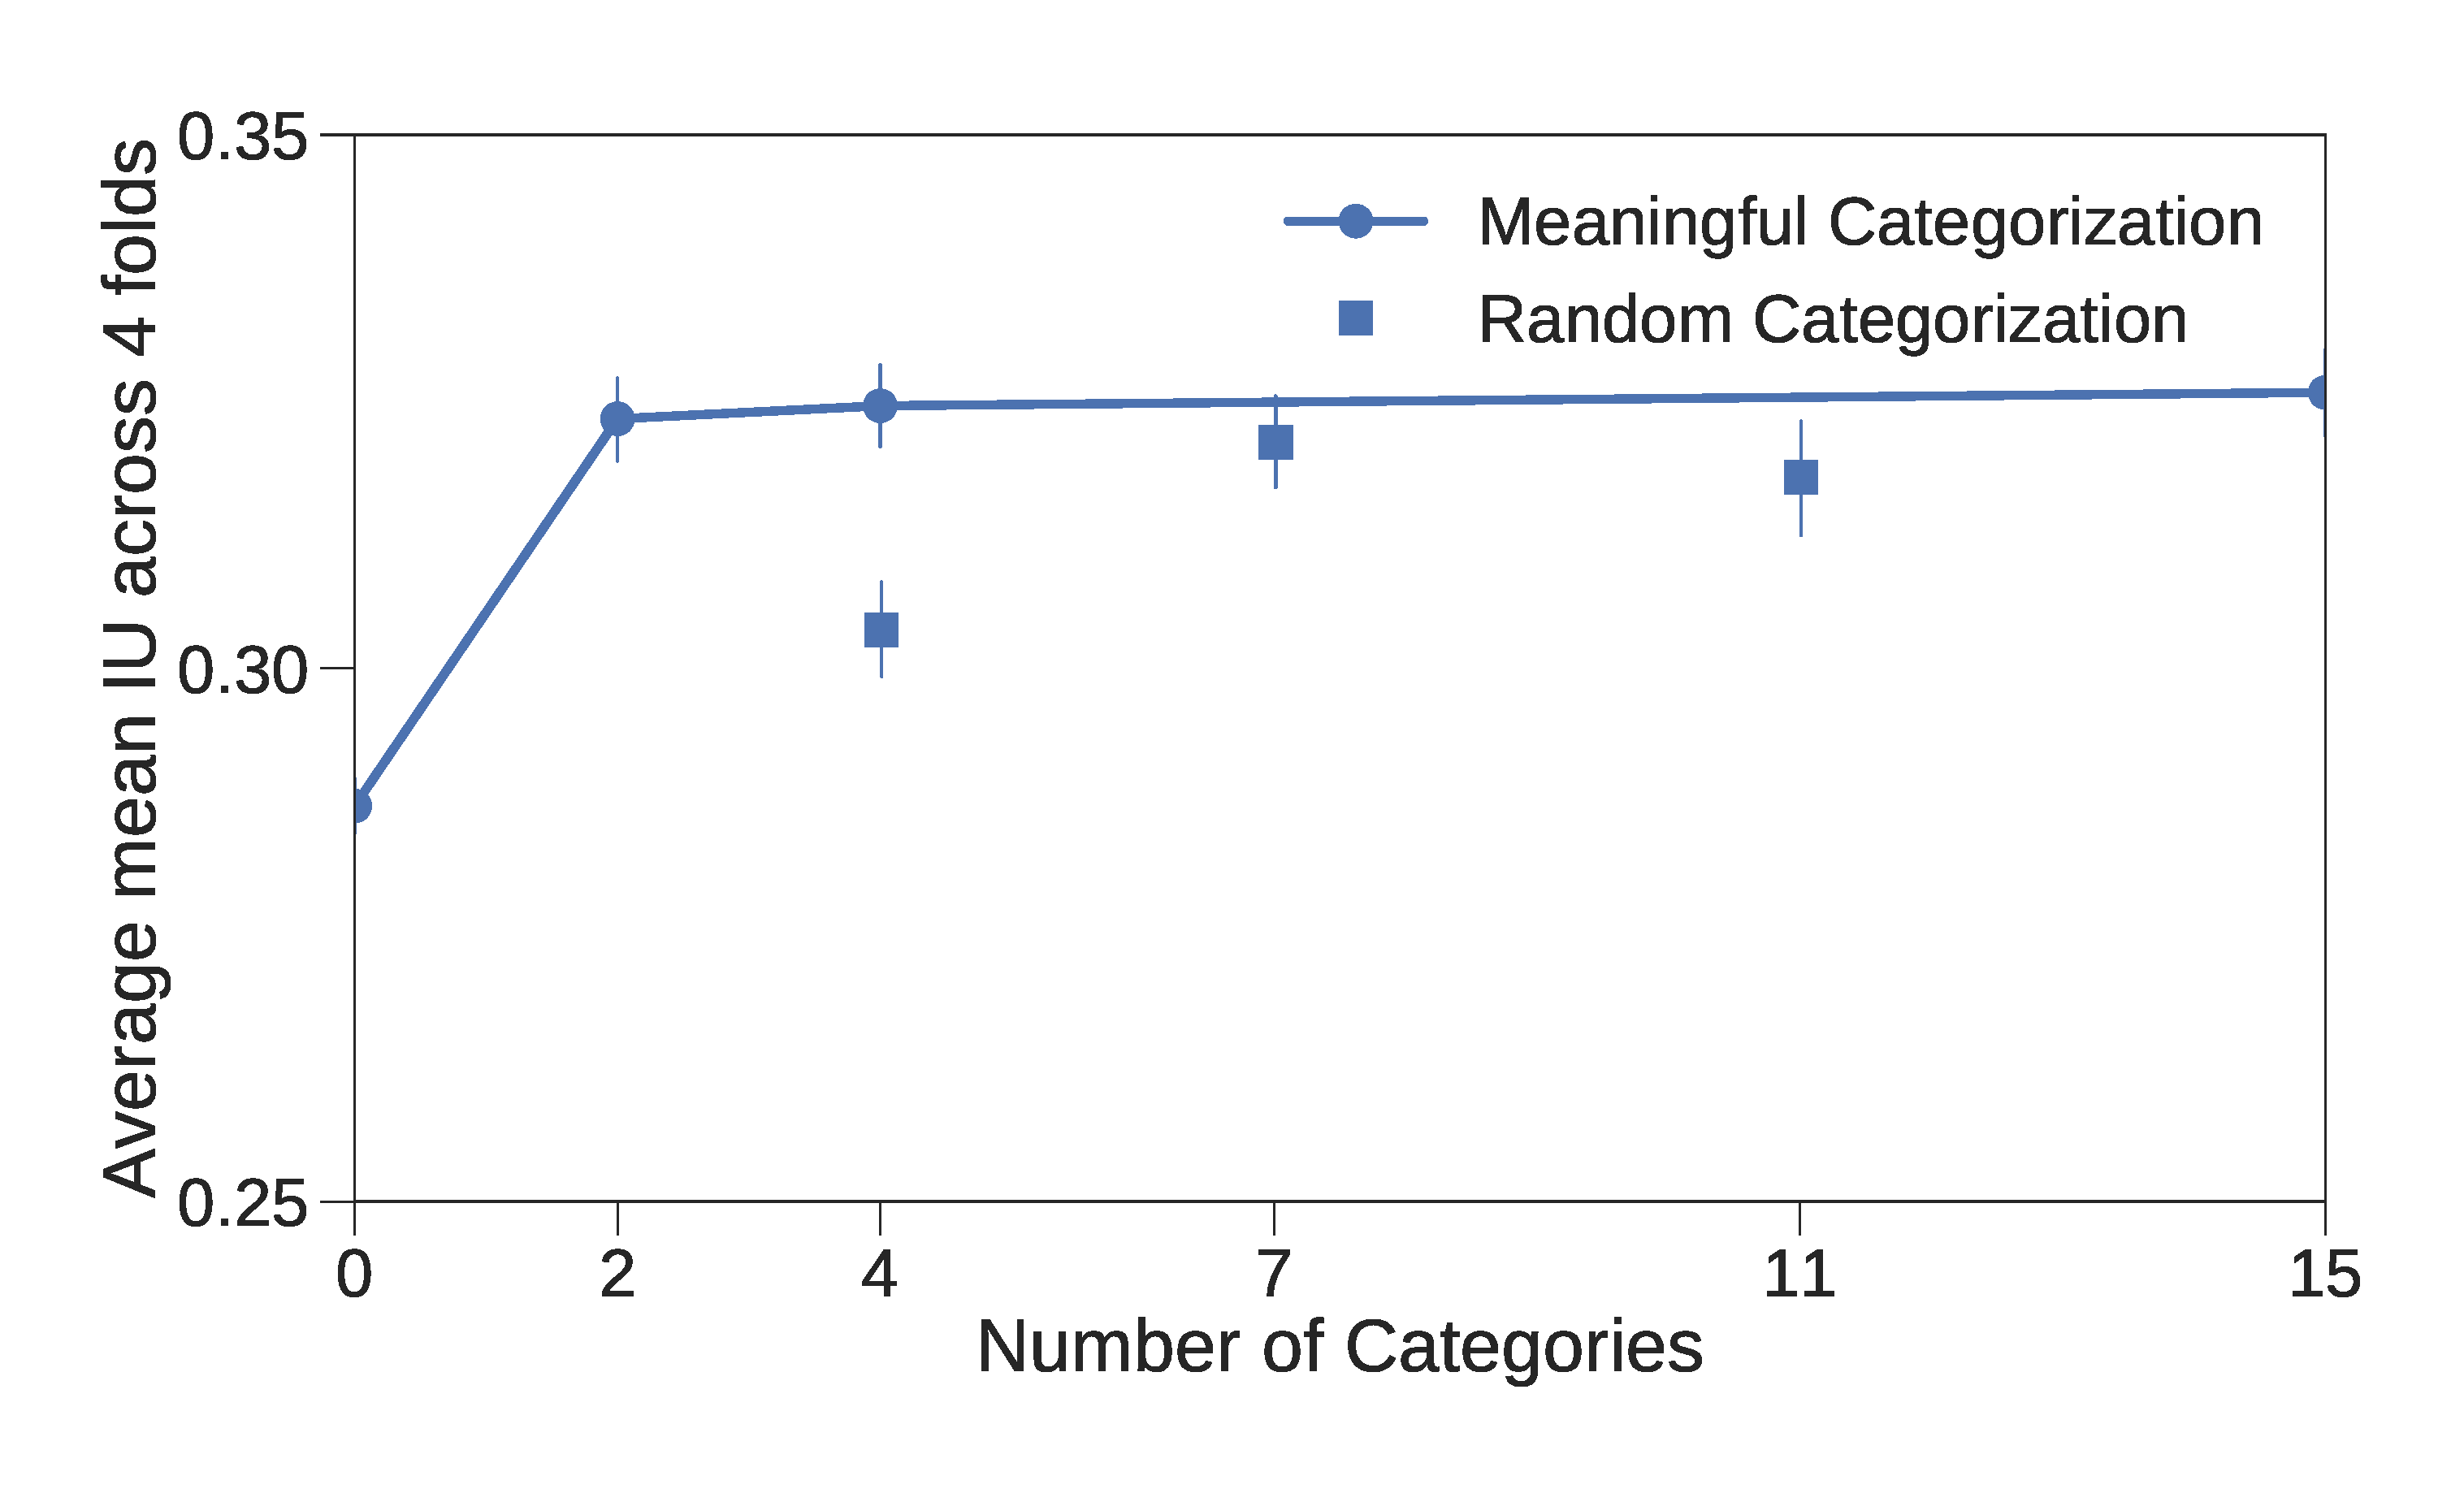
\includegraphics[width=1.\linewidth]{img/num_classes.eps}
\caption{
Segmentation performance for the fine-tuned representations learned with various categorizations of the pre-training classes.
Zero categorize means no pre-trained weights used and the model was random initialized.
Error bars located on lines denote the meaningful categorization, and isolated error bars denote random categorizations (RC) of the 15 classes.
The displayed mean IU/mean accuracies and standard deviations were averaged over four folds.
The line shows that binarizing and categorizing classes meaningful had little negative effect on the learned representations.
}
\label{fig:categories}
\end{figure}



%%%%%%%%%%%%%%%%%%%%%%%%%%%%%%%%%%%%%%%%%%%%%%%%%%%%%%%%%%%%
%%%%%%%% Table incomplete segmetation
%%%%%%%%%%%%%%%%%%%%%%%%%%%%%%%%%%%%%%%%%%%%%%%%%%%%%%%%%%%%
\begin{table*}[t]
\centering
\textbf{Fine-tuning performance of representations trained in the presence of incomplete segmentations}\par\medskip
\resizebox{\textwidth}{!}{
\centering
\begin{tabular}{l|c|cccc|c}

\hline
\multirow{2}{*}{}                                                                 & \multirow{2}{*}{\begin{tabular}[c]{@{}c@{}}Pre-trained\\ Models\end{tabular}} & \multicolumn{4}{c|}{Fine-tuning mean IU per pretraining-finetuning fold}                                                                       & \multicolumn{1}{l}{\multirow{2}{*}{\begin{tabular}[c]{@{}l@{}}Average \\ mean IU\end{tabular}}} \\ \cline{3-6}
                                                                                  &                                                                               & \multicolumn{1}{l}{Fold1}         & \multicolumn{1}{l}{Fold2}         & \multicolumn{1}{l}{Fold3}         & \multicolumn{1}{l|}{Fold4}         & \multicolumn{1}{l}{}                                                                            \\ \hline
\multirow{2}{*}{Baseline}                                                         & RandomWeights                                                                 & $0.29\pm0.01$                     & $0.29\pm0.03$                     & $0.27\pm0.01$                     & $0.30\pm0.02$                      & $0.29\pm0.02$                                                                                   \\
                                                                                  & CompleteLabels                                                                    & \multicolumn{1}{c}{$0.29\pm0.01$} & \multicolumn{1}{c}{$0.36\pm0.01$} & \multicolumn{1}{c}{$0.29\pm0.01$} & \multicolumn{1}{c|}{$0.37\pm0.01$} & \multicolumn{1}{c}{$\mathbf{0.33\pm0.01}$}                                  \\ \hline
\multirow{2}{*}{\begin{tabular}[c]{@{}l@{}}Inexaustive\\ Segmention\end{tabular}} & HalfUnsegmented                                                               & $0.26\pm0.01$                     & $0.30\pm0.03$                     & $0.28\pm0.03$                     & $0.32\pm0.02$                      & $0.29\pm0.02$                                                                                   \\
                                                                                  & SigmoidalLoss                                                                 & \multicolumn{1}{l}{$0.30\pm0.01$} & \multicolumn{1}{l}{$0.37\pm0.01$} & \multicolumn{1}{l}{$0.31\pm0.02$} & \multicolumn{1}{l|}{$0.34\pm0.02$} & $\mathbf{0.33\pm0.02}$                                                                          \\ \hline

\end{tabular}
}
\caption{
Segmentation performance for FCN-AlexNet models pre-trained on 15 categories from the PASCAL VOC2011 dataset and fine-tuned on the other five categories.
The splits of pre-training and fine-tuning categories are organized in four folds.
\textbf{RandomWeights} represents the randomly initialized weights;
\textbf{CompleteLabels} stands for the model pre-trained with complete segmentations;
\textbf{HalfUnsegmented} denotes the model pre-trained with half of the objects unsegmented;
\textbf{SigmoidLoss} means that the model pre-trained with half of the objects unsegmented and with the sigmoid loss applied to the background class.
Applying the sigmoid loss to the negative class when pre-trained with inexhaustive segmentations achieves a fine-tuning performance comparable to pre-training with the complete segmentations, better than training with the normal logistic loss.
}
\label{tab:unseg}
\end{table*}


%%%%%%%%%%%%%%%%%%%%%%%%%%%%%%%%%%%%%%%%%%%%%%%%%%%%%%%%%%%%
%%%%%%%% Table False positive segmentations
%%%%%%%%%%%%%%%%%%%%%%%%%%%%%%%%%%%%%%%%%%%%%%%%%%%%%%%%%%%%
\begin{table*}[t]
\centering
\textbf{Fine-tuning performance of representations trained in the presence of false positive segmentations}\par\medskip
\resizebox{\textwidth}{!}{
\centering
\begin{tabular}{l|c|cccc|c}

\hline
\multirow{2}{*}{}                                                               & \multirow{2}{*}{\begin{tabular}[c]{@{}c@{}}Pre-trained\\ Models\end{tabular}} & \multicolumn{4}{c|}{Fine-tuning mean IU per pretraining-finetuning fold}                                                                       & \multirow{2}{*}{\begin{tabular}[c]{@{}l@{}}Average \\ mean IU\end{tabular}} \\ \cline{3-6}
                                                                                &                                                                               & Fold1                             & Fold2                             & Fold3                             & Fold4                              &                                                                             \\ \hline
\multirow{2}{*}{Baseline}                                                       & RandomWeights                                                                 & \multicolumn{1}{c}{$0.29\pm0.01$} & \multicolumn{1}{c}{$0.29\pm0.03$} & \multicolumn{1}{c}{$0.27\pm0.01$} & \multicolumn{1}{c|}{$0.30\pm0.02$} & \multicolumn{1}{c}{$0.29\pm0.02$}                                           \\
                                                                                & NoFalsePositive                                                    & $0.26\pm0.01$                                                                                           & $0.37\pm0.03$                                                                               & $0.27\pm0.01$                                                                                                  & $0.33\pm0.04$                                                                                           & $\mathbf{0.31\pm0.02}$                                                                                                 \\ \hline
False positive segmentaion                                                      & HalfFalsePositive                                                  & \multicolumn{1}{l}{$0.27\pm0.01$}                                                                       & \multicolumn{1}{l}{$0.34\pm0.01$}                                                           & \multicolumn{1}{l}{$0.30\pm0.01$}                                                                              & \multicolumn{1}{l|}{$0.32\pm0.01$}                                                                      & $\mathbf{0.31\pm0.01}$                                                                                                 \\ \hline

\end{tabular}
}
\caption{
Segmentation performance for FCN-AlexNet models pre-trained on 15 categories from the PASCAL VOC2011 dataset and fine-tuned on the other five categories.
The splits of pre-training and fine-tuning categories are organized in four folds.
\textbf{RandomWeights} represents the randomly initialized weights;
\textbf{NoFalsePositive} denotes the model pre-trained with no segmented object from the non-relevant categories;
\textbf{HalfFalsePositive} represents the model pre-trained with segmented objects from the noninterested categories;
Including the false positive segmentations in pre-training achieves no worse fine-tuning performance than not including the false positive segmentations, better than random initialization.
}
\label{tab:falsepos}
\end{table*}


%%%%%%%%%%%%%%%%%%%%%%%%%%%%%%%%%%%%%%%%%%%%%%%%%%%%%%%%%%%%
\subsection{Learning representaions in the presence of mislabeled segmentations}
\label{subsec:robustness}
%%%%%%%%%%%%%%%%%%%%%%%%%%%%%%%%%%%%%%%%%%%%%%%%%%%%%%%%%%%%

%%%%%%%% TEXT Experiment setup

To learn representations in the presence of lablel errors, we set up three experiments for three types of label errors, (1) inexhaustive segmentations, (2) objects mislabelling and (3) false positive segmentations, independently with three datasets constructed from a well-annotated dataset, the PASCAL VOC2011 segmentation dataset \cite{everingham2015pascal}.


\subsubsection{Datasets}
\label{subsubsec:noises}

In this experiment, fifteen out of twenty categories of the VOC2011 dataset were selected to form a \textit{pre-training dataset} and the other categories formed a \textit{fine-tuning dataset}.
% The pre-training dataset was used to learn representations by training to segment objects.
% The fine-tuning dataset was used to fine-tune the learned representations.
Three types of label errors of interest were introduced independently with stochastical corruptions to the well-annotated pre-training dataset.
To avoid the influence of the choice of the pre-training and fine-tuning splitting for categories, we divided the 20 categories of VOC2011 equally into four folds.
The exact folds of categories are:
\begin{description}
  \item [Fold 1] aeroplane, bicycle, bird, boat, bottle
  \item [Fold 2] bus, car, cat, chair, cow
  \item [Fold 3] dining table, dog, horse, motorbike, person
  \item [Fold 4] potted plant, sheep. sofa, train, TV
\end{description}
The training dataset was enriched with extra segmentations by Hariharan et al. \cite{hariharan2011semantic}
To keep the segmentation task simple, we used only single-object images, resulting in totally 4000 training images for 20 categories available for pre-training, fine-tuning and evaluation.
The original images were subsampled by four times to accelerate the training process.



\subsubsection{Experimental setup}
\label{subsubsec:ptft}
A Fully Convolutional Network with AlexNet (FCN-AlexNet) model \cite{long2015fully}, as shown in Table \ref{fig:fcn} in Appendix \ref{subsec:segmentation}, was used for segmentation.
Models were first pre-trained with the pre-training datasets and then fine-tuned with the fine-tuning datasets.
The fine-tuned models were evaluated by mean intersection over union ratio (mean IU) on the fine-tuning test set, which is referred to as the \textit{fine-tuning performance}.
Performance improvement of fine-tuning transferred models compared to a randomly initialized model indicates the transferability of pre-trained weights.
The non-transferable layers of FCN-AlexNet were randomly initialized with Xavier Initialization.
% The pre-trained AlexNet model was used to set a baseline of performance, denoted as the ImageNet model.
Random weights initialization were considered as the baseline.
A well pre-trained model should at least outperform random weights initialization.
The default hyperparameters of FCN-AlexNet in  \cite{long2015fully} were kept unchanged.
The training process run 240,000 iterations for pre-training phase, and 12,000 iterations for fine-tuning phase.
Snapshots for trained models were taken every 4,000 iterations.
Each experiment was repeated three times, mean and standard deviation were computed over the last five snapshots for all repetitions.

% \noindent \textit{What Table \ref{tab:robustness} tell us.
% How annotation errors were synthesized;
% How synthesizations are different from reality;
% Transferability of noisy models compared to clean models.
% }


\subsubsection{Results}


%%%%%%%%%%%%%%%%%%%%%%%%%%%%%%%%%%%%%%%%%%%%%%%%%%%%%%%%%%%%
%%%%%%%%%% Objects mislabeling
%%%%%%%%%%%%%%%%%%%%%%%%%%%%%%%%%%%%%%%%%%%%%%%%%%%%%%%%%%%%

\paragraph{Training binary segmentations in the presence of objects mislabelling}
Objects Mislabelling denotes that a subset of segmented objects are mislabeled from one category to another in a training segmentation dataset.
To validate that training binary segmentation can learn representations better than training per-category segmentation in the presence of objects mislabelling, we constructed three different datasets with (1) all random labels for objects, (2) half random and half correct labels for objects, and (3) all correct labels for objects.
The learned representations with these three datasets were fine-tuned to segment the five fine-tuning categories and evaluated by a test set for the five fine-tuning classes.

Results in Table \ref{tab:random} suggests that pre-training with mislabeled foreground objects have a negative influence on the learned representations.
Compared to the model trained with true labels, both models trained with all random labels and half-true half-random foreground labels do not present improvement of segmentation performance to the random weights initialization on the test set of the fine-tuning dataset.

We instead discard the labels for the objects and train binary (foreground/background) segmentation.
The result representations achieve a fine-tuning performance better than training with the mislabeled objects and equivalent to the model pre-trained with correct labels.
Randomized object labels were mislabeled among foreground classes so that binarizing labels a foreground and background classes can in a sense correct the randomized labels.
% Compared to the precise but inaccurate noisy labels, binarized labels are accurate but imprecise.
This observation indicates that binarizing segmentation labels into foreground and background have little influence on the learned representations.

\paragraph{Categorizing the foreground classes}
We then investigate the influence of categorizing the foreground classes instead of grouping all of them as one foreground class.
We categorized the fifteen pre-training classes into four meaningful categories: person, animal, vehicle, indoor according to \cite{everingham2015pascal}, and trained segmentation models to transfer.
The fifteen pre-training classes were also randomly categorized into 4, 7, 11 categories, respectively, to pre-train segmentation models.
The learned multi-categories segmentation models are then fine-tuned with the 5-categories fine-tuning dataset and shown as the error bars in Figure \ref{fig:categories}.

The line in Figure \ref{fig:categories} demonstrates that the segmentations labeled in one category, in four categories, and in fifteen categories have no significant influence on the learned representations.
All the three learned representations improve the fine-tuning performance compared to a random weights initialization show as the blue circle at categories=0.
Additionally, the isolated error bars in figure \ref{fig:categories} reveal that even training by random categorization of the foreground classes has little effect on the fine-tuning performance for the learned representations.
This observation indicates that it is not necessary to group the foreground classes into meaningful categories to reserve the class specific information.
Therefore, we propose to train foreground/background segmentations when the purpose is to learn representations that can transfer to another dataset.

\paragraph{Training with the sigmoid loss applied to the background class in the presence of inexhaustive segmentation}
Inexhaustive segmentation means that there exist unsegmented objects of interest in the training images.
To validate the use of sigmoid loss for the background class can alleviate the negative effects of inexhaustive segmentation to the learned representation, we constructed a training dataset with only 50\% of the objects segmented, together with a training dataset with 100\% of the objects segmented.
Segmented means the object is labeled as foreground, and unsegmented means the object is labeled as background.
The class-dependent sigmoid loss and the normal logistic loss were applied to the dataset with 50\% of the objects unsegmented.
The learned representations were evaluated by fine-tuned and validated with the five-categories fine-tuning dataset.

The segmentation performance, mean IU, for the model pre-trained with incomplete segmentations is worse than the model pre-trained with complete segmentations by 0.04 when using the logistic loss to train, are demonstrated in Table \ref{tab:unseg}.
By applying the class-dependent sigmoid loss to pre-train models with half of the objects unsegmented, the learned representations achieve a fine-tuning performance comparable to the model pre-trained with complete segmentation.
The representations learned with the class-dependent sigmoid loss is demonstrated to achieve better fine-tuning performance than the normal logistic loss.
% The negative influence of inexhaustive segmentations on the fine-tuning performance of the pre-traine model is compensated.
% The details of implementing sigmoid negative loss for the pre-training dataset will be discussed in Section \ref{subsec:pulearning}.



\paragraph{Including false positive segmentations for training if they present}
False positive segmentations represents those segmented objects that are semantically meaningful but not from a pre-defined category to segment.
To investigate the influence of including false positive segmentations for training, we consider a dataset contains dogs as the only category to segment.
Objects from the other fourteen categories are not supposed to be segmented for an error-free dataset without false positive segmentations.
The model trained with this correctly labeled dataset is named as the NoFalsePositive model in Table \ref{tab:falsepos}.
Another dataset, containing half of the objects from the other fourteen categories segmented, is referred to as the HalfFalsePositive model.

We observe, as presented in Table \ref{tab:falsepos}, that transferring the HalfFalsePositive model performs almost the same as the NoFalsePositive model and better than the random weights initialization.
Based on this observation, we conclude that including the false positive segmentations for training have little negative effects on the learned CNN representations.
% The exact influence of false segmentations in practice, however, may depend on how similar the target and non-target categories are, or whether false segmentations are consistent, which requires further investigation.


%%%%%%%%%%%%%%%%%%%%%%%%%%%%%%%%%%%%%%%%%%%%%%%%%%%%%%%%%%%%
%%%%%%%% Deprecated big table.
%%%%%%%%%%%%%%%%%%%%%%%%%%%%%%%%%%%%%%%%%%%%%%%%%%%%%%%%%%%%
%
% \begin{table*}[t]
% \resizebox{\textwidth}{!}{
% \centering
% \begin{tabular}{l|l|llll|l}
%
% \hline
%                                                                                       & \begin{tabular}[c]{@{}c@{}}Initial Feature\\ Extractor\end{tabular} & \multicolumn{4}{c|}{Fine-tuning mean IU per pretraining-finetuning fold}                                                                                                                                                                                                                                                                                                                                                                     & \multicolumn{1}{l}{\multirow{2}{*}{\begin{tabular}[c]{@{}l@{}}Average \\ mean IU\\ across \\ four folds\end{tabular}}} \\ \cline{1-6}
% \begin{tabular}[c]{@{}l@{}}Fine-tuning\\ categories\end{tabular}                      &                                                                     & \multicolumn{1}{l}{\begin{tabular}[c]{@{}l@{}}aeroplane, \\ bicycle, bird,\\ boat, bottle\end{tabular}} & \multicolumn{1}{l}{\begin{tabular}[c]{@{}l@{}}bus, car, \\ cat, \\ chair, cow\end{tabular}} & \multicolumn{1}{l}{\begin{tabular}[c]{@{}l@{}}dining table,\\ dog, horse, \\ motorbike,\\ person\end{tabular}} & \multicolumn{1}{l|}{\begin{tabular}[c]{@{}l@{}}potted plant, \\ sheep, sofa, \\ train, TV\end{tabular}} & \multicolumn{1}{l}{}                                                                                                   \\ \hline
% \multirow{2}{*}{\begin{tabular}[c]{@{}l@{}}Baseline\end{tabular}} & ImageNetModel                                                       & $0.42\pm0.01$                                                                                           & $0.51\pm0.01$                                                                               & $0.49\pm0.01$                                                                                                  & $0.47\pm0.01$                                                                                           & $0.47\pm0.01$                                                                                                          \\
%                                                                                       & RandomWeights                                                       & $0.29\pm0.01$                                                                                           & $0.29\pm0.03$                                                                               & $0.27\pm0.01$                                                                                                  & $0.30\pm0.02$                                                                                           & $0.29\pm0.02$                                                                                                          \\ \hline
% \multirow{4}{*}{\begin{tabular}[c]{@{}l@{}}Objects \\ Mislabelling\end{tabular}}       & TrueLabels                                                      & $0.29\pm0.01$                                                                                           & $0.36\pm0.01$                                                                               & $0.29\pm0.01$                                                                                                  & $0.37\pm0.01$                                                                                           & $\mathbf{0.33\pm0.01}$                                                                                                 \\
%                                                                                       & AllRandomLabels                                                     & $0.29\pm0.01$                                                                                           & $0.33\pm0.03$                                                                               & $0.26\pm0.01$                                                                                                  & $0.28\pm0.01$                                                                                           & $0.29\pm0.01$                                                                                                          \\
%                                                                                       & HalfRandomLabels                                                    & $0.27\pm0.01$                                                                                           & $0.33\pm0.02$                                                                               & $0.25\pm0.01$                                                                                                  & $0.29\pm0.01$                                                                                           & $0.29\pm0.01$                                                                                                          \\
%                                                                                       & BinarizedLabels                                                     & $0.30\pm0.02$                                                                                           & $0.35\pm0.01$                                                                               & $0.29\pm0.02$                                                                                                  & $0.35\pm0.03$                                                                                           & $\mathbf{0.32\pm0.02}$                                                                                                 \\ \hline
% \multirow{3}{*}{\begin{tabular}[c]{@{}l@{}}Inexaustive \\ segmention\end{tabular}}    & CompleteLabels                                                      & $0.29\pm0.01$                                                                                           & $0.36\pm0.01$                                                                               & $0.29\pm0.01$                                                                                                  & $0.37\pm0.01$                                                                                           & $\mathbf{0.33\pm0.01}$                                                                                                 \\
%                                                                                       & HalfUnsegmented                                                     & $0.26\pm0.01$                                                                                           & $0.30\pm0.03$                                                                               & $0.28\pm0.03$                                                                                                  & $0.32\pm0.02$                                                                                           & $0.29\pm0.02$                                                                                                          \\
%                                                                                       & SigmoidLoss                                                       & \multicolumn{1}{l}{$0.30\pm0.01$}                                                                       & \multicolumn{1}{l}{$0.37\pm0.01$}                                                           & \multicolumn{1}{l}{$0.31\pm0.02$}                                                                              & \multicolumn{1}{l|}{$0.34\pm0.02$}                                                                      & $\mathbf{0.33\pm0.02}$                                                                                                 \\ \hline
% \multirow{2}{*}{\begin{tabular}[c]{@{}l@{}}False positive \\ segmentaion\end{tabular}}         & NoFalsePositive                                                    & $0.26\pm0.01$                                                                                           & $0.37\pm0.03$                                                                               & $0.27\pm0.01$                                                                                                  & $0.33\pm0.04$                                                                                           & $\mathbf{0.31\pm0.02}$                                                                                                 \\
%                                                                                       & HalfFalsePositive                                                  & \multicolumn{1}{l}{$0.27\pm0.01$}                                                                       & \multicolumn{1}{l}{$0.34\pm0.01$}                                                           & \multicolumn{1}{l}{$0.30\pm0.01$}                                                                              & \multicolumn{1}{l|}{$0.32\pm0.01$}                                                                      & $\mathbf{0.31\pm0.01}$                                                                                                 \\ \hline
%
% \end{tabular}
% }
% \caption{
% Segmentation performance for fine-tuned FCN-AlexNet models pre-trained on 15 categories from the PASCAL VOC2011 dataset and fine-tuned on the other 5 categories.
% \textbf{ImageNetModel} represents the pre-trained ImageNet model;
% \textbf{RandomWeights} indicates that the randomly initialized weights;
% All the other extractors were pre-trained in the presence/absence of the corresponding label noises listed in the leftmost column.
% Half of the objects unsegmented (\textbf{HalfUnsegmented}) result in pre-trained models not better than random weight initialization.
% Introducing the sigmoid negative loss in the pre-training phase was able to improve the fine-tuning performance to be comparable to pre-trained model with complete segmentation (\textbf{CompleteLabels}).
% Using random labels (\textbf{RamdomLabels}) decreased the fine-tuning performance of transferred models, compared to using true labels (\textbf{TrueLabels}).
% Binarizing the pre-training classes as foreground and background help overcome the negative effects of random labels.
% Applying the sigmoid loss to the negative class when pre-trained with inexhaustive segmentations achieves a comparable fine-tuning performance to pre-training with the complete segmentations.
% Including the false positive segmentations in pre-training (\textbf{HalfFalsePositive}) achieves the same fine-tuning performance as not including the false positive segmentations (\textbf{NoFalsePositive}), better than random initialization.
% % \textit{SingleCategory} was pre-trained on only one annotated category, either ``dog'' or ``cat'' depending on the fold, and the other categories were left unannotated;
% % \textit{BinaryLabels} was pre-trained with binary labels that any objects of the fifteen categories were annotated as one single category, namely ``dog'' or ``cat'' depending on fold;
% % \textit{TrueLabels} was pre-trained with all objects segmented and assigned to 15 categories correctly;
% % \textit{AllRandomLabels} was pre-trained with all objects correctly segmented but assigned random labels;
% % \textit{HalfRandomLabels} was pre-trained with all objects correctly segmented and half of them randomly assigned labels;
% % \textit{IncompleteLabels} was trained with datasets that objects were annotated correctly with a probability of 0.5;
% }
% \label{tab:robustness}
% \end{table*}
%
